\chapter{Resultados}
\label{cap:resultados}

Este cap\'itulo presenta los resultados de las cinco variantes y los relaciona con las
hip\'otesis formuladas en el \cref{sec:planteamiento}. El an\'alisis comienza con la
cobertura de las ejecuciones, contin\'ua con la evoluci\'on del rendimiento y de las
p\'erdidas, y concluye con una comparaci\'on cualitativa y las limitaciones de la evidencia.

\section{Cobertura de las ejecuciones}
\label{sec:cobertura-resultados}

La \cref{tab:resultados} resume la cobertura de los registros y el mejor valor de la
m\'etrica principal. V0 y V1 agotaron \num{500} \'epocas, V2 complet\'o \num{266}, V3
registr\'o \num{155} y V4 agot\'o su presupuesto de \num{200}. Los dos transformadores
solo disponen de cuatro evaluaciones, frente a las diez de V0 y V1.

\begin{table}[htbp]
  \centering
  \caption{Cobertura de los entrenamientos y mejor puntuaci\'on media de evaluaci\'on.}
  \label{tab:resultados}
  \small
  \begin{tabular}{llrrrcr}
    \toprule
    Variante & Estrategia & \'Epocas & Eval. & Mejor puntuaci\'on & IC \SI{95}{\percent} &
      \'Epoca \\
    \midrule
    V0 & Desde cero  & \num{500} & \num{10} & \num{0.864} $\pm$ \num{0.040} &
      {[\num{0.787};\,\num{0.942}]} & \num{350} \\
    V1 & Congelado   & \num{500} & \num{10} & \num{0.668} $\pm$ \num{0.053} &
      {[\num{0.564};\,\num{0.771}]} & \num{150} \\
    V2 & Ajuste fino & \num{266} & \num{6}  & \num{0.648} $\pm$ \num{0.057} &
      {[\num{0.536};\,\num{0.759}]} & \num{150} \\
    V3 & Congelado   & \num{155} & \num{4}  & \num{0.622} $\pm$ \num{0.053} &
      {[\num{0.518};\,\num{0.727}]} & \num{100} \\
    V4 & Congelado   & \num{200} & \num{4}  & \num{0.535} $\pm$ \num{0.059} &
      {[\num{0.419};\,\num{0.651}]} & \num{100} \\
    \bottomrule
  \end{tabular}
  \notatabla{La puntuaci\'on se acompa\~na de su error est\'andar sobre los \num{50}
    episodios evaluados. En V2 se excluye la \'epoca de \'indice \num{266}, interrumpida
    tras cinco lotes y sin validaci\'on. V3 se detuvo en el \'indice \num{154}.}
  \fuente{elaboraci\'on propia}
\end{table}

El valor reportado es el m\'aximo de una serie de evaluaciones y, por tanto, un estimador
optimista. La media de las tres \'ultimas ofrece una lectura menos sesgada: \num{0.862} en
V0, \num{0.547} en V1, \num{0.585} en V2, \num{0.572} en V3 y \num{0.483} en V4. V0
permanece estable, mientras que las cuatro variantes preentrenadas retroceden despu\'es de
su m\'aximo. El sesgo del m\'aximo puede favorecer a V0 y V1 porque acumulan m\'as
evaluaciones; la media final mantiene, no obstante, la ventaja de V0.

V2 se reanud\'o desde un punto de control intermedio. El registro conserva tanto cinco
\'epocas de la rama abandonada como sus equivalentes tras la reanudaci\'on, con pasos
globales repetidos. Para construir las curvas se mantuvo la primera sesi\'on hasta la
\'epoca \num{69} y la rama reanudada desde la \num{70}. Este criterio evita promediar
estados del optimizador que no pertenecen a una misma trayectoria de entrenamiento.

\section{Evoluci\'on del rendimiento}
\label{sec:evolucion-rendimiento}

La \cref{fig:evolucion-score} representa exclusivamente las evaluaciones oficiales sobre
las \num{50} condiciones reservadas. Las barras verticales indican el error est\'andar de
la media sobre esos episodios. Los marcadores se sit\'uan cada \num{50} \'epocas y
las estrellas identifican el punto de control seleccionado para cada variante.

\begin{figure}[htbp]
  \centering
  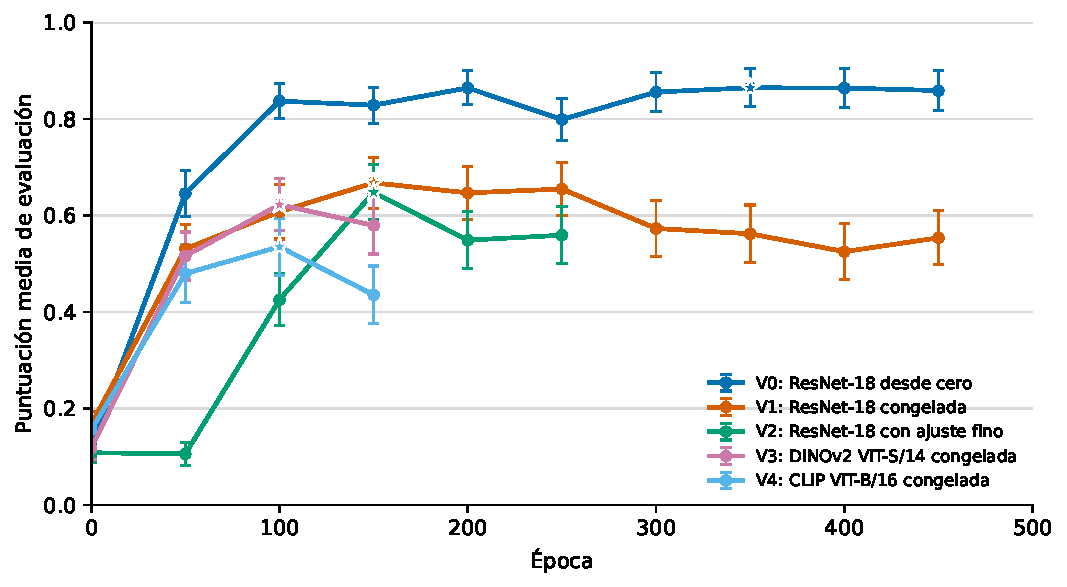
\includegraphics[width=0.92\textwidth]{img/evolucion_puntuacion_prueba.pdf}
  \caption{Evoluci\'on de la puntuaci\'on media de evaluaci\'on de las cinco variantes.}
  \label{fig:evolucion-score}
  \fuente{elaboraci\'on propia}
\end{figure}

V0 alcanza \num{0.8370} en la \'epoca \num{100} y permanece cerca de \num{0.86} durante
la mayor parte del entrenamiento posterior. Su m\'aximo, \num{0.8645}, aparece en la
\'epoca \num{350}; la \'ultima evaluaci\'on, en la \num{450}, conserva \num{0.8588}. La
peque\~na diferencia entre ambos valores indica que la selecci\'on del punto de control no
depende de un pico aislado.

V1 mejora hasta \num{0.6676} en la \'epoca \num{150}. Despu\'es oscila brevemente alrededor
de \num{0.65} y desciende hasta \num{0.5536} en la \'ultima evaluaci\'on. Esta reducci\'on
equivale a \num{0.1140} puntos, un \num{17.1}\,\% respecto a su m\'aximo. En consecuencia,
las \num{350} \'epocas restantes no producen un punto de control mejor.

V2 presenta una convergencia m\'as lenta. Su puntuaci\'on permanece alrededor de
\num{0.11} hasta la \'epoca \num{50}, asciende a \num{0.4253} en la \num{100} y alcanza
\num{0.6477} en la \num{150}. Las dos evaluaciones posteriores caen a \num{0.5487} y
\num{0.5590}. Este comportamiento motiva la detenci\'on anticipada, puesto que prolongar
la ejecuci\'on no hab\'ia recuperado el m\'aximo tras \num{100} \'epocas.

V3 progresa de \num{0.1177} a \num{0.6224} entre las \'epocas \num{0} y \num{100}. La
evaluaci\'on de la \'epoca \num{150} desciende a \num{0.5792}, y la ejecuci\'on se detiene
cuatro \'epocas despu\'es. V4 alcanza \num{0.5351} en la \'epoca \num{100} y cae a
\num{0.4353} en la \num{150}, antes de completar las \num{200} \'epocas asignadas.

La comparaci\'on de los mejores puntos de control sit\'ua V0 por encima de las dem\'as
variantes. Los m\'argenes abarcan desde \num{0.197} frente a V1 hasta \num{0.329} frente a
V4. La \cref{tab:contrastes} relaciona las diez diferencias con su dispersi\'on entre
episodios y con el contraste de Wilcoxon.

\begin{table}[htbp]
  \centering
  \caption{Diferencias pareadas entre los puntos de control seleccionados.}
  \label{tab:contrastes}
  \small
  \scriptsize
  \begin{tabular}{lcccc}
    \toprule
    Comparaci\'on & Diferencia media & IC \SI{95}{\percent} & $p$ & $p_{\mathrm{Holm}}$ \\
    \midrule
    V0 frente a V1 & \num{0.197} & {[\num{0.091};\,\num{0.303}]} & \num{0.0004} & \num{0.0030} \\
    V0 frente a V2 & \num{0.217} & {[\num{0.102};\,\num{0.332}]} & \num{0.0001} & \num{0.0009} \\
    V0 frente a V3 & \num{0.242} & {[\num{0.122};\,\num{0.362}]} & \num{0.0003} & \num{0.0026} \\
    V0 frente a V4 & \num{0.329} & {[\num{0.208};\,\num{0.451}]} & \num{0.000003} & \num{0.000030} \\
    V1 frente a V2 & \num{0.020} & {[\num{-0.093};\,\num{0.133}]} & \num{0.82} & \num{1.00} \\
    V1 frente a V3 & \num{0.045} & {[\num{-0.089};\,\num{0.179}]} & \num{0.46} & \num{1.00} \\
    V1 frente a V4 & \num{0.132} & {[\num{0.018};\,\num{0.247}]} & \num{0.0084} & \num{0.0501} \\
    V2 frente a V3 & \num{0.025} & {[\num{-0.101};\,\num{0.152}]} & \num{0.54} & \num{1.00} \\
    V2 frente a V4 & \num{0.113} & {[\num{-0.034};\,\num{0.259}]} & \num{0.10} & \num{0.5154} \\
    V3 frente a V4 & \num{0.087} & {[\num{-0.027};\,\num{0.201}]} & \num{0.14} & \num{0.5532} \\
    \bottomrule
  \end{tabular}
  \notatabla{Diferencias calculadas sobre los \num{50} episodios comunes. La prueba de
    Wilcoxon emplea la aproximaci\'on normal y los diez valores $p$ se ajustan mediante el
    procedimiento de Holm. Los intervalos no incorporan este ajuste.}
  \fuente{elaboraci\'on propia}
\end{table}

Las cuatro diferencias entre V0 y las variantes preentrenadas excluyen el cero y conservan
significaci\'on tras el ajuste de Holm. Entre las variantes preentrenadas, solo V1 frente a
V4 alcanza significaci\'on sin corregir, con $p = \num{0.0084}$. El ajuste eleva ese valor
a \num{0.0501}, por lo que ning\'un contraste interno supera el umbral familiar del
\SI{5}{\percent}. Estos resultados no cuantifican la variabilidad entre semillas de
entrenamiento, cuesti\'on que se retoma en el \cref{sec:limitaciones}.

\section{Ajuste y generalizaci\'on}
\label{sec:ajuste-resultados}

La puntuaci\'on de la tarea debe interpretarse junto con las p\'erdidas del modelo. La
\cref{fig:evolucion-perdidas} muestra los valores agregados al final de cada \'epoca
completa. La escala logar\'itmica permite observar simult\'aneamente la fase inicial y los
cambios de menor magnitud al final del entrenamiento.

\begin{figure}[htbp]
  \centering
  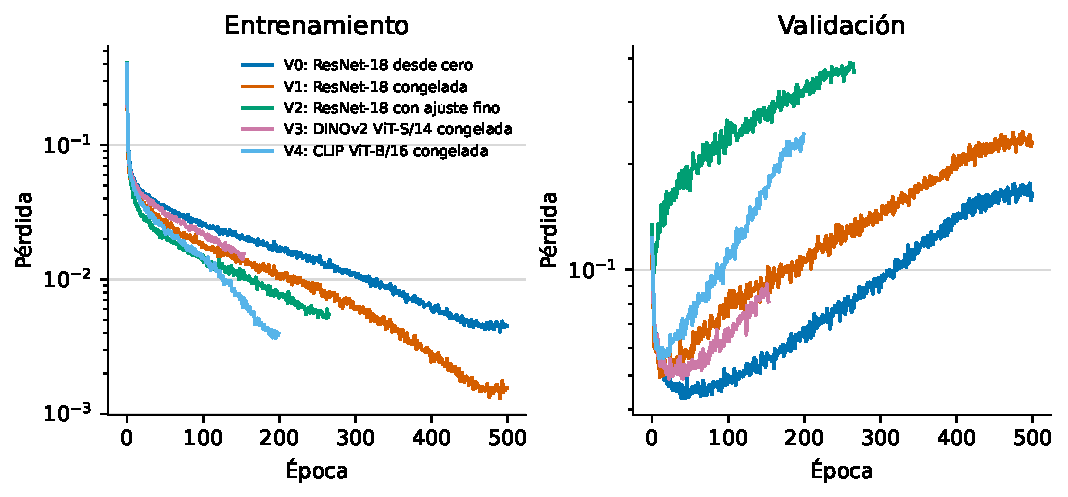
\includegraphics[width=0.95\textwidth]{img/evolucion_perdidas.pdf}
  \caption{Evoluci\'on de las p\'erdidas de entrenamiento y validaci\'on.}
  \label{fig:evolucion-perdidas}
  \fuente{elaboraci\'on propia}
\end{figure}

Las cinco variantes reducen de forma sostenida la p\'erdida de entrenamiento. Sin embargo,
la p\'erdida de validaci\'on vuelve a crecer despu\'es de las primeras \'epocas. El patr\'on
es especialmente claro en V1: entre las \'epocas \num{150} y \num{450}, la p\'erdida de
entrenamiento baja de \num{0.0145} a \num{0.00166}, mientras que la de validaci\'on sube
de \num{0.0869} a \num{0.2247} y la puntuaci\'on de evaluaci\'on disminuye.

V2 muestra la misma divergencia. Entre las \'epocas \num{150} y \num{250}, su p\'erdida de
entrenamiento pasa de \num{0.0115} a \num{0.00587}, la de validaci\'on aumenta de
\num{0.277} a \num{0.380} y la puntuaci\'on pierde \num{0.089} puntos. Ambos casos son
compatibles con sobreajuste. V0 tambi\'en incrementa su p\'erdida de validaci\'on, pero su
puntuaci\'on permanece estable; por tanto, la p\'erdida de predicci\'on del ruido no act\'ua
como sustituto directo del rendimiento en bucle cerrado.

V3 y V4 reproducen esa divergencia. Entre las \'epocas \num{100} y \num{150}, la p\'erdida
de entrenamiento de V3 baja de \num{0.0218} a \num{0.0155}, mientras la de validaci\'on
sube de \num{0.0681} a \num{0.0865}. En V4, las mismas magnitudes pasan de \num{0.0143} a
\num{0.00741} y de \num{0.110} a \num{0.171}. Ambas puntuaciones disminuyen a la vez.

El error cuadr\'atico medio de la acci\'on refuerza esa distinci\'on. En los puntos de
control seleccionados vale \num{116.17} para V0, \num{147.31} para V1, \num{42.86} para
V2, \num{314.78} para V3 y \num{94.93} para V4. V2 obtiene el menor error, pero no la
mejor puntuaci\'on. La precisi\'on sobre acciones registradas y el control en bucle cerrado
miden, por tanto, propiedades diferentes.

\section{Coste computacional}
\label{sec:coste-resultados}

Los tiempos recogidos en la \cref{tab:coste} muestran diferencias amplias. El bucle de V0
requiere \SI{1.6}{\minute} por \'epoca, frente a \SI{5.3}{\minute} en V1,
\SI{14.7}{\minute} en V2, \SI{2.3}{\minute} en V3 y \SI{4.0}{\minute} en V4. Estos valores
multiplican el coste de la l\'inea base por factores entre \num{1.5} y \num{9.5}.

V2 a\~nade la retropropagaci\'on a trav\'es del codificador y presenta el mayor coste por
\'epoca. V4 duplica las actualizaciones debido a su lote de \num{32} muestras. V3 muestra,
sin embargo, que operar a \num{224} p\'ixeles no determina por s\'i solo el tiempo: su
codificador congelado queda m\'as cerca de V0 que de V1.

Conviene no confundir ese coste unitario con el tiempo total. V2 acumula \SI{84.9}{\hour}
frente a las \SI{96.5}{\hour} de V1 pese a ser la variante m\'as cara por \'epoca, porque
se detuvo antes. V3 solo suma \SI{10.9}{\hour} por la misma raz\'on. La comparaci\'on v\'alida
entre variantes es el tiempo por \'epoca; el total de \SI{237.1}{\hour} describe el
experimento ejecutado con presupuestos distintos.

\section{Comprobaci\'on cualitativa}
\label{sec:resultados-cualitativos}

Los cuadernos de inferencia permiten inspeccionar trayectorias individuales de los mejores
puntos de control. La \cref{fig:inferencia-v1-v2} compara V1 y V2 desde la misma condici\'on
inicial, generada con la semilla \num{10049}. Cada panel muestra el estado inicial, el
estado final y la puntuaci\'on instant\'anea durante el episodio.

\begin{figure}[!t]
  \centering
  \begin{subfigure}{0.98\textwidth}
    \centering
    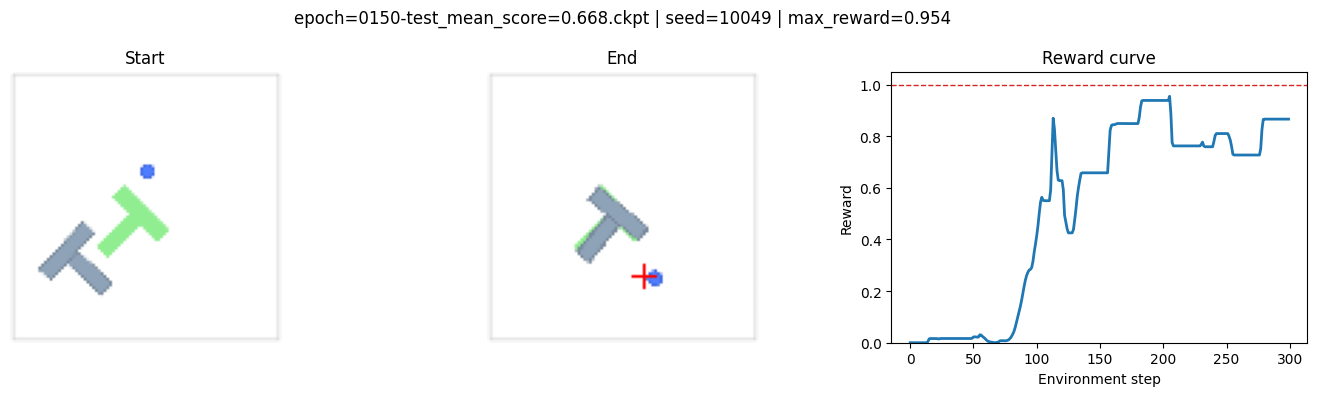
\includegraphics[width=\linewidth]{img/inferencia_v1.png}
    \caption{V1, ResNet-18 preentrenada y congelada.}
    \label{fig:inferencia-v1}
  \end{subfigure}

  \vspace{6pt}

  \begin{subfigure}{0.98\textwidth}
    \centering
    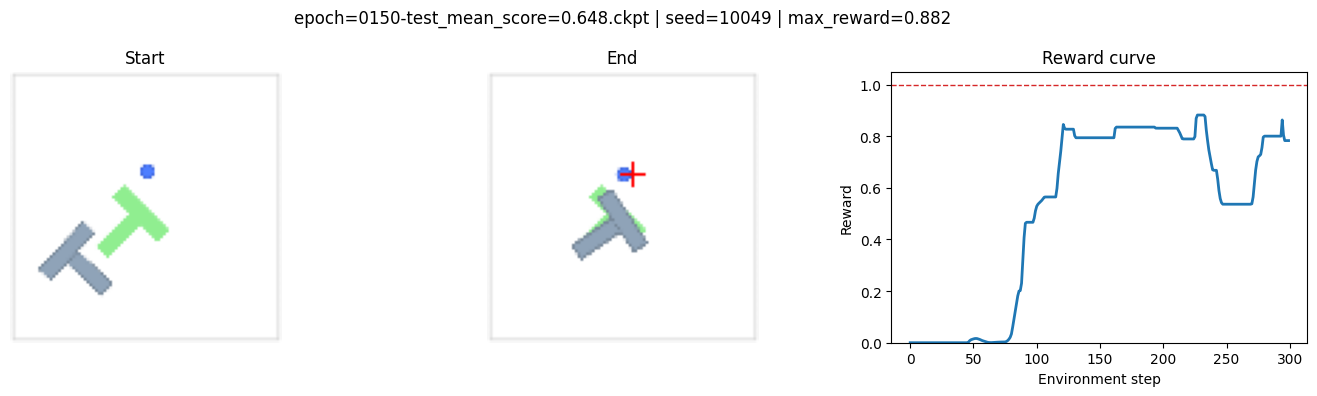
\includegraphics[width=\linewidth]{img/inferencia_v2.png}
    \caption{V2, ResNet-18 preentrenada con ajuste fino.}
    \label{fig:inferencia-v2}
  \end{subfigure}
  \caption{Inferencia de V1 y V2 sobre una condici\'on inicial compartida.}
  \label{fig:inferencia-v1-v2}
  \fuente{elaboraci\'on propia}
\end{figure}

V1 alcanza una puntuaci\'on m\'axima de \num{0.9544}, frente a \num{0.8818} en V2. Ninguna
de las dos trayectorias llega al umbral unitario de \'exito, aunque V1 consigue una
superposici\'on mayor. V0 s\'i alcanza \num{1.0} en su cuaderno, pero parte de la semilla
\num{10000}; por ese motivo, su trayectoria no se incorpora a la comparaci\'on visual.

Estas demostraciones no sustituyen la evaluaci\'on cuantitativa. Sus semillas quedan fuera
del intervalo oficial \num{100000}--\num{100049} y cada imagen representa un solo episodio.
Adem\'as, la puntuaci\'on mostrada es el m\'aximo temporal, no el valor del estado final.
Su funci\'on es ilustrar el comportamiento que origina la m\'etrica, no estimar el
rendimiento medio.

\section{Contraste de las hip\'otesis}
\label{sec:contraste-hipotesis}

La primera hip\'otesis planteaba que el preentrenamiento aportar\'ia representaciones m\'as
\'utiles que el entrenamiento desde cero. Los resultados no la respaldan: V0 supera entre
\num{0.197} y \num{0.329} puntos a las cuatro variantes preentrenadas. Todas las
diferencias conservan significaci\'on tras el ajuste de Holm.

La segunda hip\'otesis propon\'ia una ventaja del ajuste fino sobre la congelaci\'on. Tampoco
queda respaldada, ya que V1 obtiene \num{0.668} y V2 \num{0.648}. La diferencia de
\num{0.020} no alcanza significaci\'on ($p = \num{0.82}$) y su intervalo de confianza,
{[\num{-0.093};\,\num{0.133}]}, contiene el cero. En consecuencia, tampoco cabe afirmar la
superioridad de la congelaci\'on: lo que descarta la evidencia es una mejora observable del
ajuste fino en esta ejecuci\'on.

La tercera hip\'otesis propon\'ia que los transformadores alcanzar\'ian un rendimiento
comparable al de las redes convolucionales con mayor coste de inferencia. V3 y V4 quedan
por debajo de V0, pero no se distinguen de V1 y V2 tras la correcci\'on familiar. Por tanto,
los datos no muestran una ventaja de rendimiento propia de la arquitectura ViT. La parte
relativa a inferencia no puede contrastarse porque no se midi\'o su latencia bajo un
protocolo com\'un.

\section{Limitaciones}
\label{sec:limitaciones}

La primera limitaci\'on es la desigualdad del presupuesto de \'epocas. V0 y V1 acumulan
diez evaluaciones, V2 seis, y V3 y V4 solo cuatro. V3 se interrumpi\'o tras \num{155}
\'epocas de las \num{300} previstas, de modo que no puede descartarse una recuperaci\'on
posterior. La comparaci\'on corresponde a los mejores puntos observados dentro de esos
presupuestos, no a curvas con igual horizonte.

La segunda limitaci\'on es el uso de una sola semilla de entrenamiento. Los intervalos y
los contrastes de la \cref{tab:contrastes} cuantifican la dispersi\'on debida a las
condiciones iniciales del simulador, ya que los \num{50} episodios son condiciones
distintas evaluadas con el mismo modelo. No cuantifican, en cambio, la variabilidad entre
ejecuciones de entrenamiento, puesto que cada variante se ha ajustado una sola vez. Una
r\'eplica con otra semilla podr\'ia desplazar las curvas, y esa incertidumbre queda fuera
de las cifras reportadas.

La tercera afecta a la selecci\'on del modelo. Las \num{50} condiciones reservadas se
eval\'uan peri\'odicamente y determinan qu\'e punto de control se conserva, de modo que
act\'uan como conjunto de selecci\'on y no como evaluaci\'on final independiente, tal como
precisa el \cref{sec:metricas}. El m\'aximo reportado presenta por ello un sesgo optimista,
que la media de las tres \'ultimas evaluaciones ayuda a acotar. Cerrar el problema
exigir\'ia evaluar los puntos de control seleccionados sobre un bloque de semillas disjunto
del empleado en la selecci\'on, medida que no se ha ejecutado y que se propone en el
\cref{sec:trabajo-futuro}.

Por \'ultimo, la evaluaci\'on cada \num{50} \'epocas ofrece una visi\'on discreta de la
trayectoria y puede omitir m\'aximos intermedios. V2 a\~nade una reanudaci\'on, y solo su
tiempo acumulado requiere extrapolaci\'on parcial. Estas restricciones aconsejan
interpretar las cifras como evidencia del experimento realizado, no como una ordenaci\'on
universal de los codificadores.
